\documentclass{article}
\usepackage[utf8]{inputenc}
\usepackage{amsmath}
\usepackage{amssymb}
\usepackage{amsthm}
\usepackage{cancel}
\usepackage[shortlabels]{enumitem}
\usepackage{caption}
\usepackage{graphicx}
\usepackage[top=0.5in, bottom=0.5in, left=1in, right=1in]{geometry}
\usepackage{float}

% \usepackage{titlesec}
%     \titlespacing{\subsection}{\parindent}{15pt}{12pt}

\title{\textbf{\underline{CSCI4030U: Big Data Analytics}\\Lab06}}
\author{Syed Naqvi\\100590852}
\date{\today}

\begin{document}

    \maketitle

    \subsection*{1.}
    
    \begin{enumerate}[label = (\alph*), left=10pt, itemsep=10pt]
        
        \item \begin{minipage}[t]{0.9\textwidth}
            \begin{figure}[H]
                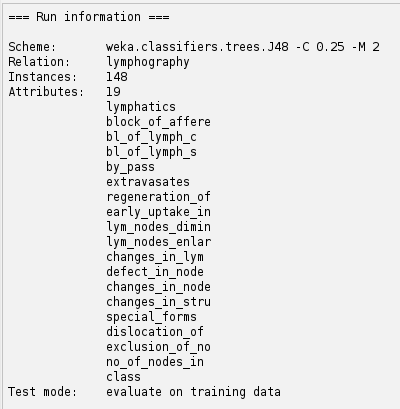
\includegraphics[width=0.5\textwidth, height=0.2\textheight]{./6ai1.png}\\
                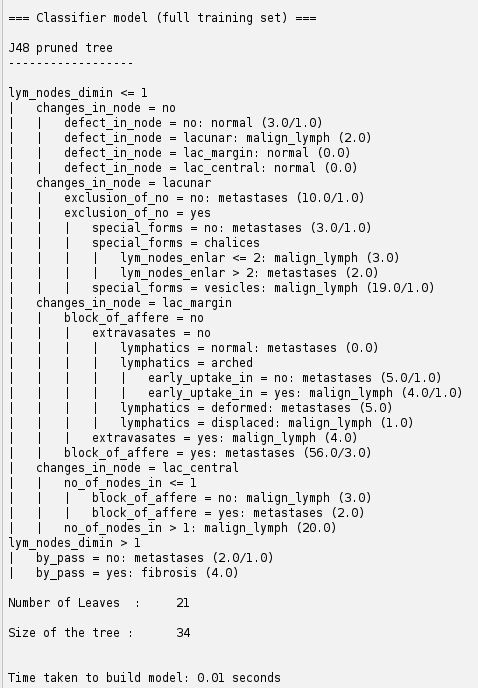
\includegraphics[width=0.6\textwidth, height=0.3\textheight]{./6aii1.png}\\
                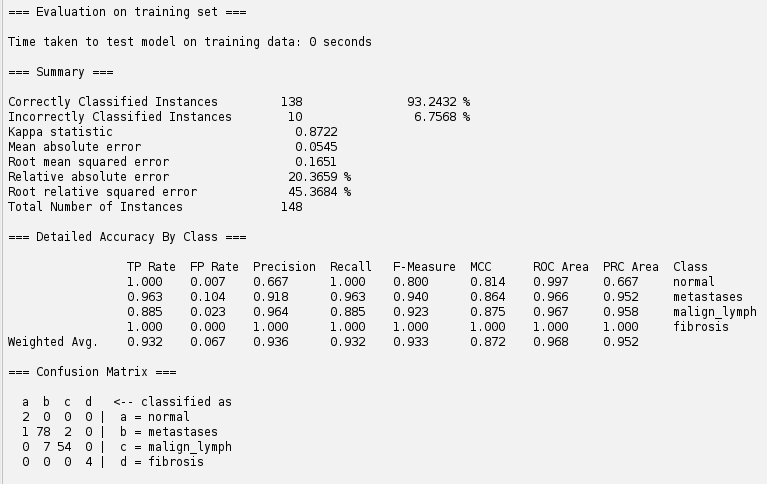
\includegraphics[width=0.6\textwidth, height=0.3\textheight]{./6aiii1.png}                
            \end{figure}
            The weka J48 algorithm is an open source version of the C4.5 algorithm which is essentially a statistical
            classification method. It creates a decision tree by using the principals of information entropy to recursively
            partitioning the dataset based on the attributes with the highest information gain. Once the tree has been
            constructed, it is pruned by removing branches that have little to no contribution to the classification
            accuracy as a result of minial information gain. Once pruning has completed, the algorithm then converts
            the decision tree into a set of if-then rules to simplify representation.
        \end{minipage}

        \item \begin{minipage}[t]{0.9\textwidth}
            \begin{figure}[H]
                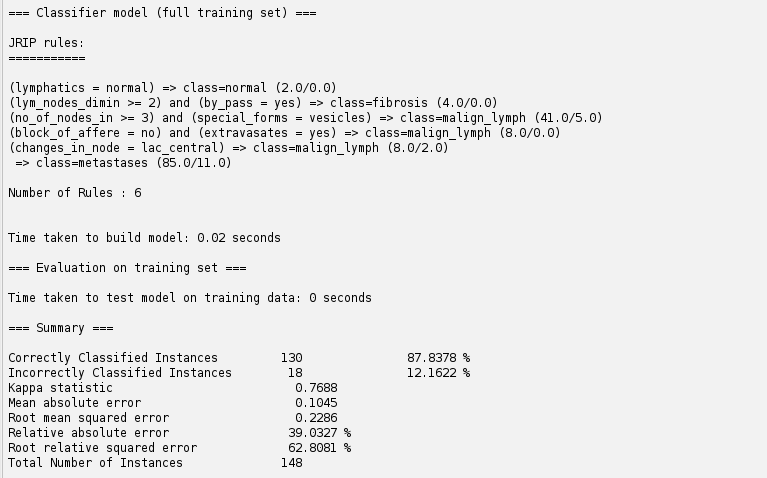
\includegraphics[width=0.5\textwidth, height=0.2\textheight]{./6bi1.png}\\
                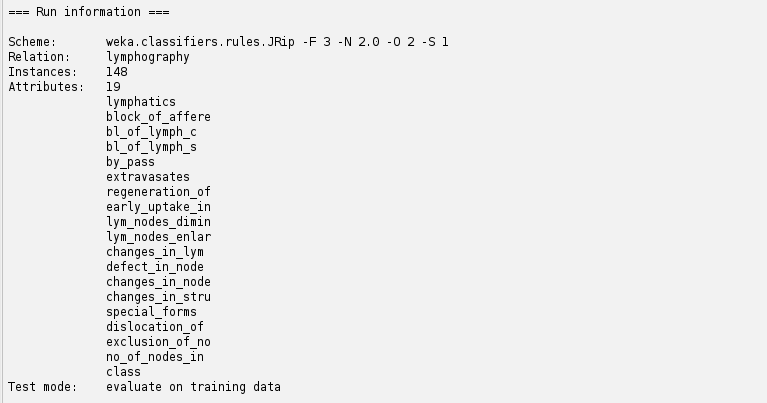
\includegraphics[width=0.6\textwidth, height=0.3\textheight]{./6bii1.png}\\
                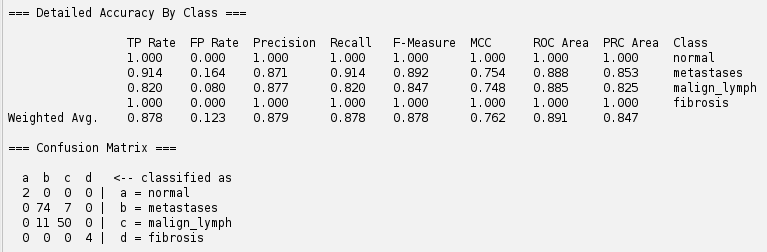
\includegraphics[width=0.6\textwidth, height=0.15\textheight]{./6biii1.png}                
            \end{figure}
            The weka JRip algorithm is an implementation of the RIPPER (Repeated Incremental Pruning to Produce
            Error Reduction) algorithm. This is a rule based classification method that iteratively constructs a set
            of if-then rules to classify data. Initially the rules are grown by adding conditions to minimize the Error
            on the training set followed by a pruning process where rules are removed to eliminate overfitting and improve
            generalization. This method is repeated for each class treating multi-class classification as a series of
            binary problems that are optimized by removing or replacing rules in order to improve overall accuracy.
            The final model consists of a sequence of easy to understand rules that can be used to classify new instances.
        \end{minipage}

    \end{enumerate}

    \subsection*{2.}
    
    \begin{enumerate}[label = (\alph*), left=10pt, itemsep=10pt]
        
        \item \begin{minipage}[t]{0.9\textwidth}
            \textbf{C4.5 (weka.classifier.trees.J48)}\\
             Classification Accuracy: 97.2222\%\\
             Confusion matrix:\\
             \begin{figure}[H]
                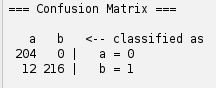
\includegraphics[width=0.3\textwidth, height=0.1\textheight]{./6a2.png}
            \end{figure}
            Just as in the previous part of this lab, the J48 algorithm creates a decision tree partitioning
            on attributes with the highest information gain. Once a decision tree has been created, it is pruned
            to remove any branches with nominal contribution to classification accuracy. The final tree 
            is then used to classify new instances. 
        \end{minipage}
        \item \begin{minipage}[t]{0.9\textwidth}
            \textbf{RIPPER (weka.classifier.rules.JRip)}\\
             Classification Accuracy: 90.2778\%\\
             Confusion matrix:\\
             \begin{figure}[H]
                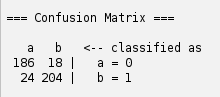
\includegraphics[width=0.3\textwidth, height=0.1\textheight]{./6b2.png}
            \end{figure}
            This algoritm first generates a set of if-then rules seeking to minimize classification error by adding as many
            conditions as possible. It then prunes the rules to reduce over-fitting and increase generalization. This process
            is repeated for each class and the result is a straight-forward set of rules that can be used to classify new
            instances.
        \end{minipage}
        \item \begin{minipage}[t]{0.9\textwidth}
            \textbf{k-Nearest Neighbor (weka.classifiers.lazy.IBk)}\\
             Classification Accuracy: 87.5\%\\
             Confusion matrix:\\
             \begin{figure}[H]
                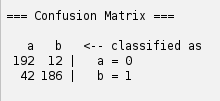
\includegraphics[width=0.3\textwidth, height=0.1\textheight]{./6c2.png}
            \end{figure} 
            This algorithm stores the training dataset in memory and calcualtes the distance
            (could be euclidean or manhattan or something else) between a new instance and its 'k'
            closest neighbours. The instance is then assigned the class most common amongst its neighbours. 
        \end{minipage}
        \item \begin{minipage}[t]{0.9\textwidth}
            \textbf{Naive Bayesian Classification (weka.classifiers.bayes.NaiveBayes)}\\
             Classification Accuracy: 97.2222\%\\
             Confusion matrix:\\
             \begin{figure}[H]
                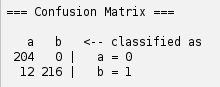
\includegraphics[width=0.3\textwidth, height=0.1\textheight]{./6d2.png}
            \end{figure} 
            This algorithm makes strong independence assumptions between features and uses Bayes' theorem
            to determine the probability of a class given a set of input features. It then uses the features of an
            unseen instance to determine the most likely class. 
        \end{minipage}
        \item \begin{minipage}[t]{0.9\textwidth}
            \textbf{Neural Networks (weka.classifiers.functions.MultilayerPerceptron)}\\
             Classification Accuracy: 93.5185\%\\
             Confusion matrix:\\
             \begin{figure}[H]
                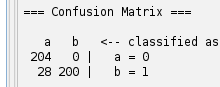
\includegraphics[width=0.3\textwidth, height=0.1\textheight]{./6e2.png}
            \end{figure}
            This algorithm is an implementation of a feedforward ariticial neural network where each neuron in one layer
            connects to every neuron in the next layer. Features in the training data are passed through the the layers
            and processed via weighted connections and activation functions to produce a prediction. The prediction is then
            compared to the actual output and then back propagated through the network to adjust the weights
            in reverse and minimize error in the case of a new instance.
        \end{minipage}

    \end{enumerate}

\end{document}